\documentclass[orivec]{llncs}
\usepackage{graphicx}
\usepackage{amsmath}			% for "cases"
\usepackage{amsfonts}		% for frakur fonts
\usepackage{mathrsfs}		% for curly "E" error symbol
\usepackage{float}
\usepackage[most]{tcolorbox}	% for wrapping example in color box
% \usepackage{wrapfig}			% wrap figure beside text, used in example
\usepackage{tikz-cd}			% commutative diagrams
\usepackage{tikz}
\usepackage{amssymb}			% for \multimap \updownarrow \bigstar \varnothing
\usepackage{sectsty}			% change section color
% \usepackage{turnstile}		% longer turnstiles
\usepackage{wasysym}			% smileys
\usepackage[normalem]{ulem}	% underline with line breaks: /uline
\usepackage{hyperref}		% refs, links become clickable
\usepackage[]{algorithm2e}	% algorithms

\usepackage{geometry}		% change paper size
\geometry{
  a4paper,         % or letterpaper
  textwidth=18cm,  % llncs has 12.2cm
  textheight=27cm, % llncs has 19.3cm
  heightrounded,   % integer number of lines
  hratio=1:1,      % horizontally centered
  vratio=2:3,      % not vertically centered
}
\usepackage[fontsize=13pt]{scrextend}

% *************** Delete when not using Chinese or colors **********************
\usepackage{xeCJK}
\setCJKmainfont[BoldFont=SimHei,ItalicFont=KaiTi]{SimSun}
\usepackage{color}
\definecolor{cerulean}{RGB}{100,100,200}
%\newcommand{\emp}[1]{\textbf{\textcolor{Cerulean}{#1}}}
\newcommand{\emp}[1]{\textbf{#1}}
\definecolor{grey}{rgb}{0.9,0.9,0.9}  % grey

% \chapterfont{\color{blue}}  % sets colour of chapters
\sectionfont{\color{blue}} 
\subsectionfont{\color{blue}} 
\subsubsectionfont{\color{blue}} 
\setcounter{secnumdepth}{3}		% use numbers in subsubsections

\let\emptyset\varnothing			% more beautiful empty set symbol
\newcommand{\vect}[1]{\boldsymbol{#1}}
\newcommand*\sigmoid{\vcenter{\hbox{
\includegraphics{sigmoid.png}}}}
\newcommand*\KB{\vcenter{\hbox{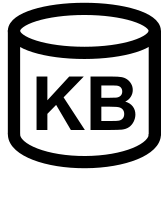
\includegraphics{KB-symbol.png}}}}
\newcommand*\NN{\vcenter{\hbox{\includegraphics{NN-symbol.png}}}}
\newcommand*\invsigmoid{\vcenter{\hbox{\includegraphics{inverse-sigmoid.png}}}}
\newcommand{\invW}{\, \rotatebox[origin=c]{90}{W}}
\newcommand{\invw}{\, \rotatebox[origin=c]{90}{w}}
\newcommand*\rectifier{\vcenter{\hbox{\includegraphics{rectifier.png}}}}
\newcommand{\dashh}{\textemdash~}
\newcommand{\tab}{\hspace*{1cm}}

\newcommand{\tikzmark}[1]{\tikz[overlay,remember picture] \node (#1) {};}

\let\labelitemi\labelitemii

\renewcommand{\thefootnote}{\fnsymbol{footnote}}
\interfootnotelinepenalty=10000

% ***** Boxed variables inside math equations
% \newcommand*{\boxedcolor}{black}
\makeatletter
% \renewcommand{\boxed}[1]{\textcolor{\boxedcolor}{%
% \fbox{\normalcolor\m@th$\displaystyle#1$}}}
% \setlength{\fboxsep}{1pt}
\renewcommand{\boxed}[1]{\fbox{\m@th$\displaystyle\scalebox{0.9}{#1}$} \,}
\makeatother

\overfullrule=0mm

\newsavebox{\MyName}
\savebox{\MyName}{
\includegraphics[scale=0.6]{YKY.png}}

\title{什么是机器学习? What is machine learning?}
\titlerunning{什么是机器学习?}
\author{\usebox{\MyName} (King-Yin Yan)
% \\ \footnotesize{General.Intelligence@Gmail.com}
}
\institute{General.Intelligence@Gmail.com}

\begin{document}

\maketitle
\setlength{\parindent}{0em}
% \setlength{\parskip}{2.8ex plus0.8ex minus0.8ex}
\setlength{\parskip}{2.8ex}

%\begin{abstract}
%\end{abstract}

机器学习是 AI 最重要部分,但我上次用 Clojure 写 Genifer 的时候没有完成这部分,结果那 prototype 完全没有应用,是一大失误。

\section{「学习」的本质}

人脑很多时是通过「一般化 , generalization」来学习的。

例如,广东话俗语说:『有须就认老窦』(有胡子便认做父亲,用来取笑过份的一般而论),但可能婴儿就是这样辨认亲人的。 

又例如,小时候爷爷教我写中文的「一二三四五」,学到 3 的时候我便自作聪明地说:「我知道了,四字的写法是 4 划!」  虽然是错误的,但表示小孩子的思想方式。

又例如,有些人被女人骗过一次之后,便永远不信女人。

这些都是 generalization 的例子。

相反的方向叫 specialization (特殊化),或 refinement (精细化)。

例如我们从「所有女人都说谎」修正到「有些女人是诚实的」,或者「那个骗我的女人其实也有诚实的一面。」 

一般化 和 特殊化 就是逻辑学习的基本运作,没有别的内容了。

此外还有一种机器学习的範畴,是基於在空间中的点的模式识别:
\begin{equation}
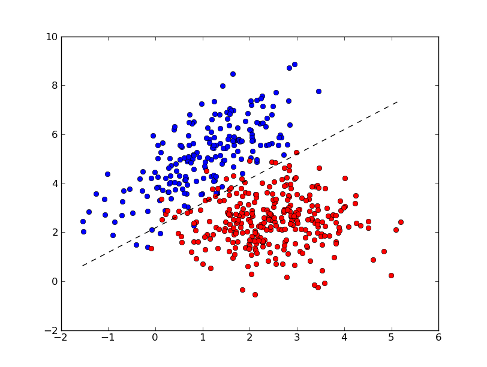
\includegraphics[scale=0.75]{pattern-recognition-linear-example.png}
\end{equation}

例如我们已经知道有两类东西 (分别标作{\color{red}红色}和{\color{blue}蓝色}),而我们数量化地量度它们的某些特徵,然后在座标空间上点描出来,这时发现{\color{red}红点}和{\color{blue}蓝点}的分布大致可以用一条线分割,於是以后我们只要量度那些特徵,就可以分辨哪些是{\color{red}红组}或{\color{blue}蓝组}的东西,而不需要知道事先知道它们的颜色(label)。

这种「空间中」的统计学习 (statistical learning),其先决条件是知道一些数值上的量度,否则根本没有几何空间可言。  神经网络就是这种 ``spatial learning'' 的例子。

On the other hand,逻辑学习是不需要几何空间的,它只需要「符号」运作 (symbolic manipulations)。 

以下我们专注逻辑学习;  如何统一逻辑学习和空间学习,我觉得是研究的重要课题。

\section{Logic-based learning}

例如说,我们观察到「很多读电脑的人都戴眼镜」,但我们是怎样跳到这个「归纳」的结论的?

在逻辑引擎中,已经有的 gound facts (事实资料) 是:
\begin{itemize}
\item 读电脑(小明), 戴眼镜(小明)
\item 读电脑(小娟), 戴眼镜(小娟)
\item 读电脑(小强), 戴眼镜(小强)
\item 读电脑(美玲), 戴眼镜(美玲)
\item 读音乐(小芬),不 戴眼镜(小芬)
\item 男生(小明),男生(小强)
\item 女生(小娟),女生(美玲),女生(小芬)
\item . . . . . . . 等等。
\end{itemize}
我们欲求得到的 general rule 是:
读电脑(X) $\rightarrow$ 戴眼镜(X)

其实那算法就是在所有可能的 formula 里面 \textbf{搜寻}。

换句话说,由最简单的 formula 开始,我们不断 generate 越来越复杂的 formulas,然后我们逐一试验这些 formulas,看看哪一条最能 \textbf{解释事实}。

最简单的 formula 就是一条「空」的命题 (什么也没有,表示一切都是真的)。

然后我们逐步添加一些逻辑项 (terms)。

例如:\\
\tab $\rightarrow$ 戴眼镜(X) \\
表示任何人都戴眼镜,但那和事实不符。

又例如:\\
\tab 女生(X) $\rightarrow$ 戴眼镜(X) \\
「所有女生都戴眼镜」,那也和事实不符。

最后我们试验:\\
\tab 读电脑(X) $\rightarrow$ 戴眼镜(X) \\
发现其机率很高 (或许有少数例外),於是接受这一假设。

换句话说,这是在「\textbf{假设空间},hypothesis space」中的搜寻。

这些 search space (搜寻空间) 的结构,形状像「树」那样不断细分下去:
\begin{equation}
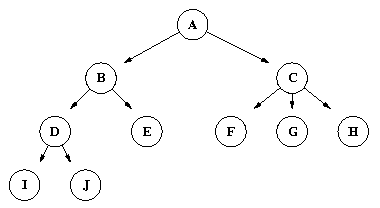
\includegraphics[scale=0.6]{search-space.png}
\end{equation}

我们由最「一般」的命题 (什么都是真的) 开始搜寻,到越来越特殊的命题,例如「22 岁、五月生日、体重 70 公斤以上、读大学 4 年级、数学不合格、姓张的人 $\rightarrow$ 都戴眼镜」,这过程中必然会出现我们期待的 formula。  这叫 general-to-specific search。

但由於 假设空间里面 有非常多 \textbf{组合} (combinatorial) 的可能性,所以这种学习是很慢的。

似乎唯一的解决之道,就是把所有概念和法则 \textbf{分类},例如「这是属於物理学的知识」、「这是关於我女朋友的知识」..... 等,而在搜寻时我们只关注那些最可能有关的集合,例如「买礼物给女友时 考虑 class A 的知识」、「物理学考试时 考虑 class B 的知识」..... 等等。

PS:  我在 Genifer 网页里有更详细地解释 \href{http://genifer.googlecode.com/files/Genifer - induction (30 July 2012).pdf}{inductive learning (PDF, in English)}。  但现在(2017)有新的想法,是用深度学习的神经网络近似整套逻辑法则的集合。 因为深度神经网络有很多层,它可以自动将不同的元素做有阶层的分类 (hierarchical classification)。

\quad \quad \quad --- 完 ---

%\bibliographystyle{plain} % or number or aaai ...
%\bibliography{AGI-book}

\end{document}
